%%%%%%%%%%%%%%%%%%%%%%%%%%%%%%%%%%%%%%%%%%%%%%%%%%%%%%%%%%%%%%%%%%%%%%%%%%%%%%%%
%% Plantilla de memoria en LaTeX para la ETSIT - Universidad Rey Juan Carlos
%%
%% Por Gregorio Robles <grex arroba gsyc.urjc.es>
%%     Grupo de Sistemas y Comunicaciones
%%     Escuela Técnica Superior de Ingenieros de Telecomunicación
%%     Universidad Rey Juan Carlos
%% (muchas ideas tomadas de Internet, colegas del GSyC, antiguos alumnos...
%%  etc. Muchas gracias a todos)
%%
%% La última versión de esta plantilla está siempre disponible en:
%%     https://github.com/gregoriorobles/plantilla-memoria
%%
%% Para obtener PDF, ejecuta en la shell:
%%   make
%% (las imágenes deben ir en PNG o JPG)

%%%%%%%%%%%%%%%%%%%%%%%%%%%%%%%%%%%%%%%%%%%%%%%%%%%%%%%%%%%%%%%%%%%%%%%%%%%%%%%%

\documentclass[a4paper, 12pt]{book}
%\usepackage[T1]{fontenc}

\usepackage[a4paper, left=2.5cm, right=2.5cm, top=3cm, bottom=3cm]{geometry}
\usepackage{times}
\usepackage[utf8]{inputenc}
\usepackage[spanish]{babel} % Comenta esta línea si tu memoria es en inglés
\usepackage{url}
%\usepackage[dvipdfm]{graphicx}
\usepackage{graphicx}
\usepackage{float}  %% H para posicionar figuras
\usepackage[nottoc, notlot, notlof, notindex]{tocbibind} %% Opciones de índice
\usepackage{latexsym}  %% Logo LaTeX

\title{Integración de una plataforma de telefonía IP}
\author{Javier Estébanez Rodríguez}

\renewcommand{\baselinestretch}{1.5}  %% Interlineado

\begin{document}

\renewcommand{\refname}{Bibliografía}  %% Renombrando
\renewcommand{\appendixname}{Apéndice}

%%%%%%%%%%%%%%%%%%%%%%%%%%%%%%%%%%%%%%%%%%%%%%%%%%%%%%%%%%%%%%%%%%%%%%%%%%%%%%%%
% PORTADA

\begin{titlepage}
\begin{center}
\includegraphics[scale=0.8]{img/URJ_logo_Color_POS.png}

\vspace{1.75cm}

\Large
Grado en Ingeniería en Sistemas Audiovisuales y Multimedia

\vspace{0.4cm}

\large
Curso Académico 2021/2022

\vspace{0.8cm}

Trabajo Fin de Grado

\vspace{2.5cm}

\LARGE
INTEGRACIÓN DE UNA PLATAFORMA DE TELEFONÍA IP

\vspace{4cm}

\large
Autor : Javier Estébanez Rodríguez \\
Tutor : Gregorio Robles Martínez
\end{center}
\end{titlepage}

\newpage
\mbox{}
\thispagestyle{empty} % para que no se numere esta pagina


%%%%%%%%%%%%%%%%%%%%%%%%%%%%%%%%%%%%%%%%%%%%%%%%%%%%%%%%%%%%%%%%%%%%%%%%%%%%%%%%
%%%% Para firmar
\clearpage
\pagenumbering{gobble}
\chapter*{}

\vspace{-4cm}
\begin{center}
\LARGE
\textbf{Trabajo Fin de Grado}

\vspace{1cm}
\large
Integración de una Plataforma de Telefonía IP

\vspace{1cm}
\large
\textbf{Autor :} Javier Estébanez Rodríguez \\
\textbf{Tutor :} Dr. Gregorio Robles Martínez

\end{center}

\vspace{1cm}
La defensa del presente Proyecto Fin de Carrera se realizó el día \qquad$\;\,$ de \qquad\qquad\qquad\qquad \newline de 2022, siendo calificada por el siguiente tribunal:


\vspace{0.5cm}
\textbf{Presidente:}

\vspace{1.2cm}
\textbf{Secretario:}

\vspace{1.2cm}
\textbf{Vocal:}


\vspace{1.2cm}
y habiendo obtenido la siguiente calificación:

\vspace{1cm}
\textbf{Calificación:}


\vspace{1cm}
\begin{flushright}
Fuenlabrada, a \qquad$\;\,$ de \qquad\qquad\qquad\qquad de 2022
\end{flushright}

%%%%%%%%%%%%%%%%%%%%%%%%%%%%%%%%%%%%%%%%%%%%%%%%%%%%%%%%%%%%%%%%%%%%%%%%%%%%%%%%
%%%% Dedicatoria

\chapter*{}
\pagenumbering{Roman} % para comenzar la numeracion de paginas en numeros romanos
\begin{flushright}
\textit{Dedicado a mi familia y a mi pareja}
\end{flushright}

%%%%%%%%%%%%%%%%%%%%%%%%%%%%%%%%%%%%%%%%%%%%%%%%%%%%%%%%%%%%%%%%%%%%%%%%%%%%%%%%
%%%% Agradecimientos

\chapter*{Agradecimientos}
%\addcontentsline{toc}{chapter}{Agradecimientos} % si queremos que aparezca en el índice
\markboth{AGRADECIMIENTOS}{AGRADECIMIENTOS} % encabezado

Aquí vienen los agradecimientos\ldots Aunque está bien acordarse de la pareja, no hay que olvidarse de dar las gracias a tu madre, que aunque a veces no lo parezca disfrutará tanto de tus logros como tú\ldots
Además, la pareja quizás no sea para siempre, pero tu madre sí.

%%%%%%%%%%%%%%%%%%%%%%%%%%%%%%%%%%%%%%%%%%%%%%%%%%%%%%%%%%%%%%%%%%%%%%%%%%%%%%%%
%%%% Resumen

\chapter*{Resumen}
%\addcontentsline{toc}{chapter}{Resumen} % si queremos que aparezca en el índice
\markboth{RESUMEN}{RESUMEN} % encabezado

El objetivo de esta memoria es presentar una solución de colaboración on-premise basada en Cisco UCS para el alojamiento de una infraestructura de telefonía IP, servicios de mensajería y Contact Center.

El sistema consiste principalmente de una centralita que gestionará la lógica de las llamadas de VoIP (Voice over Internet Protocol) con tecnología Cisco basada en Call Manager y protocolo SIP (Session Initiation Protocol).
Para hacerlo posible, se ha preparado un entorno de virtualización con la tecnología VMWare, que alojará las máquinas virtuales de la solución.

Este tipo de estructura está pensado para atender las necesidades de varias empresas (en paralelo) en cuestión de atención telefónica. La lógica que pueden esconder los distintos elementos de la arquitectura ofrece un sinfín de posibilidades, de manera que se puede llegar a realizar una gestión muy eficiente y personalizada.

%La inclusión de scripts en el Contact Center ofrece posibilidades como la aparición de una locución de bienvenida con opciones de marcado, el almacenamiento en una base de datos de las respuestas de una encuesta de satisfacción, servicios de enrutado de llamadas según demanda y asignación de colas o de agente basado en sus habilidades, entre muchas otras.
En un mundo cada vez más digitalizado, las empresas se ven obligadas a ofrecer un soporte técnico remoto ya sea telefónicamente, por chat o mediante correo electrónico. En este ámbito, la asistencia telefónica constituye una gran opción que permite mejorar la comunicación y eficiencia en la resolución de problemas, consiguiendo así un mayor grado de satisfacción en el cliente y convirtiéndose a su vez en un importante criterio de evaluación a la hora de elegir la contratación de un servicio/producto.

Empresas como Cisco, Skype o Mitel (entre otros) son grandes referentes en la implementación de estos servicios, que además permiten la comunicación interna entre trabajadores de la misma empresa sin inferir en un sobrecoste.

%%%%%%%%%%%%%%%%%%%%%%%%%%%%%%%%%%%%%%%%%%%%%%%%%%%%%%%%%%%%%%%%%%%%%%%%%%%%%%%%
%%%% Resumen en inglés

\chapter*{Summary}
%\addcontentsline{toc}{chapter}{Summary} % si queremos que aparezca en el índice
\markboth{SUMMARY}{SUMMARY} % encabezado

Here comes a translation of the ``Resumen'' into English.
Please, double check it for correct grammar and spelling.
As it is the translation of the ``Resumen'', which is supposed to be written at the end, this as well should be filled out just before submitting.


%%%%%%%%%%%%%%%%%%%%%%%%%%%%%%%%%%%%%%%%%%%%%%%%%%%%%%%%%%%%%%%%%%%%%%%%%%%%%%%%
%%%%%%%%%%%%%%%%%%%%%%%%%%%%%%%%%%%%%%%%%%%%%%%%%%%%%%%%%%%%%%%%%%%%%%%%%%%%%%%%
% ÍNDICES %
%%%%%%%%%%%%%%%%%%%%%%%%%%%%%%%%%%%%%%%%%%%%%%%%%%%%%%%%%%%%%%%%%%%%%%%%%%%%%%%%

% Las buenas noticias es que los índices se generan automáticamente.
% Lo único que tienes que hacer es elegir cuáles quieren que se generen,
% y comentar/descomentar esa instrucción de LaTeX.

%%%% Índice de contenidos
\tableofcontents
%%%% Índice de figuras
\cleardoublepage
%\addcontentsline{toc}{chapter}{Lista de figuras} % para que aparezca en el indice de contenidos
\listoffigures % indice de figuras
%%%% Índice de tablas
%\cleardoublepage
%\addcontentsline{toc}{chapter}{Lista de tablas} % para que aparezca en el indice de contenidos
%\listoftables % indice de tablas


%%%%%%%%%%%%%%%%%%%%%%%%%%%%%%%%%%%%%%%%%%%%%%%%%%%%%%%%%%%%%%%%%%%%%%%%%%%%%%%%
%%%%%%%%%%%%%%%%%%%%%%%%%%%%%%%%%%%%%%%%%%%%%%%%%%%%%%%%%%%%%%%%%%%%%%%%%%%%%%%%
% INTRODUCCIÓN %
%%%%%%%%%%%%%%%%%%%%%%%%%%%%%%%%%%%%%%%%%%%%%%%%%%%%%%%%%%%%%%%%%%%%%%%%%%%%%%%%

\cleardoublepage
\chapter{Introducción}
\label{sec:intro} % etiqueta para poder referenciar luego en el texto con ~\ref{sec:intro}
\pagenumbering{arabic} % para empezar la numeración de página con números

\section{Presentación de la solución}
\label{sec:seccion}

La implementación de esta solución se ha ideado con el objetivo de instalar un sistema de Contact Center en un cliente que de soporte a varias empresas.
Se pretende que varios agentes gestionen simultáneamente las llamadas de dichas empresas, pudiendo atender indistintamente llamadas de varios de estos orígenes.

De forma paralela, se ha provisto de un servicio de presencia (estado online, ausente, ocupado\ldots) y de mensajería interna mediante el aplicativo Finesse, apoyado en Cisco Jabber.
Mientras que Jabber proveerá del servicio de presencia, voz y monitorización silenciosa de las llamadas; Finesse será la interfaz gráfica que verá el agente, pudiendo entre otras cosas pausar y transferir llamadas o entrar en conferencias.

Adicionalmente, se ha configurado un software de terceros para la grabación de las llamadas. Desde dicho software se pueden escuchar las grabaciones y organizarlas mediante filtros, de manera que su exportación sea más controlada y proporcione datos para estadísticas.



\section{Contexto personal}
%\label{sec:seccion}
En verano del 2021 estuve plenamente implicado en un proyecto de VoIP (con la empresa en la actualmente trabajo) que me supuso un enorme reto por su complejidad, diseño inicial desde cero y las exigentes ``dead-lines'' impuestas por el cliente.

Estas circunstancias me obligaron a investigar mucho por mi cuenta sin realmente tener la posibilidad de poder apoyarme inicialmente en perfiles más completos de mi empresa al encontrarse de vacaciones.
Como suelen decir, y aunque a menudo suponga un gran esfuerzo, a veces hay que ``pegarse con ello'' para aprender y sacar las cosas adelante.
Aún contando con ayuda de mis compañeros en fases más avanzadas del proyecto, mi dedicación ha sido plena desde el inicio hasta el final, y sigue siéndolo en mejoras actuales.

La reproducción del proyecto en esta memoria me pareció idónea por su contenido tan cercano a los conocimientos adquiridos en mi grado, y a su vez me ayuda a hacer un análisis más a bajo nivel de la implementación, que me permitirá interiorizar con más precisión cada elemento configurado y su importancia dentro de la arquitectura, y así poder replicarlo en futuros proyectos.

\section{Análisis de entorno}
%\label{sec:seccion}
Tras vivir recientemente una situación límite en muchos aspectos con la pandemia de la COVID-19, el modelo de negocio actual se ha visto obligado a adaptarse para integrar el trabajo remoto en su día a día a consecuencia de las medidas de restricción sanitarias que están teniendo lugar.
Estas circunstancias han favorecido en gran medida el crecimiento de las soluciones de telefonía IP y colaboración, que ya habían sido objeto de estudio previamente por consultoras de análisis de mercados %como \textit{Market and Research} o \textit{Global Market Insights}
, arrojando unos resultados prometedores de crecimiento entre los años 2017 y 2021 y previendo la continuación de dicha tendencia en los próximos años.

Si bien las distintas soluciones de telefonía IP pretenden lograr el mismo objetivo, podemos distinguir entre los dos métodos de integración que se pueden llevar a cabo actualmente:
\begin{itemize}
  \renewcommand{\theenumi}{\alph{enumi}}
  \item \underline{On premise} o local, donde el montaje de la arquitectura se hace habitualmente en las propias instalaciones de la empresa, la cual necesita comprar, instalar y mantener el hardware. Los costes iniciales son grandes y requiere personal cualificado para su gestión, pero proporcionan un control completo y autónomo de la solución. Además, son más seguros al no tener elementos fuera de la red local por lo que el flujo de comunicación se queda dentro de la red propia.  

  \item \underline{Cloud} o en la nube, que puede ser pública o privada. La gestión y mantenimiento de la arquitectura se hace remotamente, de lo que generalmente se encarga el proveedor. Son servicios más baratos, más facilmente escalables y su puesta en marcha es mucho más rápida y sencilla, aunque impide un control total de la configuración al encontrarse supeditada a las posibilidades que of rezca el proveedor.
\end{itemize}

Para el despliegue de estas tecnologías podemos distinguir entre empresas que ofrecen productos propios vs empresas que ofrecen productos basados en tecnología de código abierto (Asterix por ejemplo), o empresas que ofrecen productos on premise\footnote{\url{https://www.gartner.com/reviews/market/contact-center-infrastructure}} frente a otras más incipientes en el mercado actual que ofrecen soluciones en cloud\footnote{\url{https://www.gartner.com/reviews/market/contact-center-as-a-service}}. Cabe hacer mención a varias empresas que ofrecen servicios de CC (Contact Center)  líderes en el sector, y representadas en años consecutivos en los famosos cuadrantes de Gartner (Figura~\ref{figura:fig_gartner}):
\begin{itemize}
  \item \textbf{Cisco.} Entre los muchos mercados en los que se encuentra, dedica al de VoIP gran parte de su atención y esfuerzo.   

  \begin{itemize}
    \item \emph{UCCX}: Unified Contact Center Express es la aplicación de centro de atención al cliente on premise que se presenta en esta memoria. Una herramienta muy potente bajo el renombre de una marca con gran reconocimiento mundial.
    \item \emph{Webex}: Muy expandida en Europa y Norte América. Ofrece un despliegue de CC en la nube con gran rapidez y flexibilidad en necesidades puntuales por sobrecarga, entre otros.
  \end{itemize}  

  \item \textbf{Mitel.} Su solución \emph{MiContact Center Business}\footnote{\url{https://www.mitel.com/es-es/productos/aplicaciones/contact-center/micontact-center-business}}, a menudo de la mano con la centralita de Call Manager MiVoice MX-ONE, es una plataforma de nivel profesional para la gestión de experiencia del cliente omnicanal, diseñada para las empresas orientadas al cliente.

  \item \textbf{Genesys}. Referente mundial en soluciones de CC y experiencia de cliente omnicanal. Presente en valoraciones Gartner de CCaaS (Contact Center as a Service) y UCaaS (Unified Communications as a Service).\\
  \\
  \\

\end{itemize}
\begin{figure}[h]
  \centering
  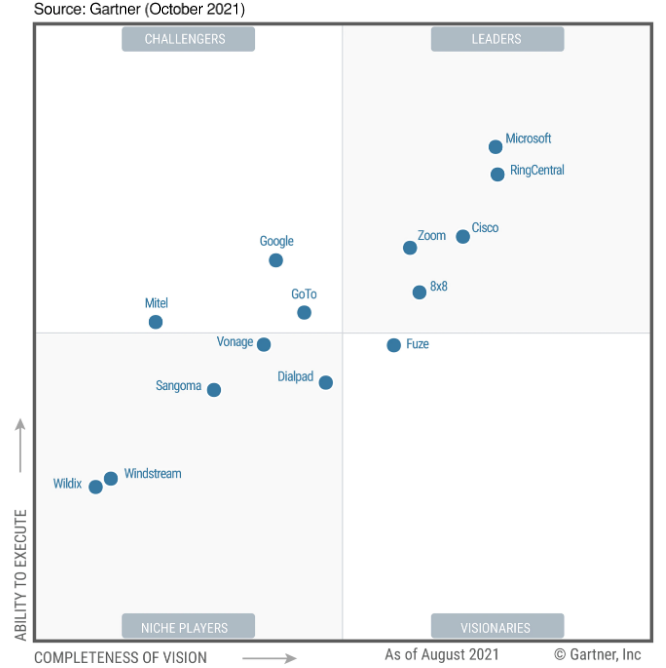
\includegraphics{img/fig_gartner_2021}
  \caption{Cuadrante mágico para UCaaS 2021}
  \label{figura:fig_gartner}
\end{figure}
En el mercado VoIP actual se está valorando cada vez más la sencillez de instalación, la interfaz, la facilidad de uso y la integración con múltiples herramientas de trabajo, además del siempre presente interés por el mayor ahorro posible dentro de unos estándares mínimos de calidad. Estos ``requisitos'' han ocasionado que emerjan soluciones de colaboración principalmente en cloud destinadas a ese propósito, pero que no ofrecen servicios de CC. Entre ellas, caben destacar dos archiconocidas en España
\begin{itemize}
  \item \textbf{Microsoft}. \emph{Teams} es la herramienta que se usa actualmente en esta universidad. Interfaz amigable, sencilla, potente y con garantías de una empresa con gran trayecto andado en este ámbito, pues podría decirse que Teams es el resultado de la evolución y muerte de Skype.  

  \item \textbf{Zoom}. No ha sido hasta la reciente pandemia que esta empresa ha ganado mayor renombre. Muy utilizada por la educación pública de España y cada vez más recurrida por empresas para satisfacer sus necesidades de comunicación, reuniones, chat, y seminarios web.
\end{itemize}
  

\section{Estructura de la memoria}
%\label{sec:seccion}

A continuación se muestra la estructura que tendrá la memoria:
\begin{itemize}
  \item En el primer capítulo se presenta el contexto personal, motivaciones de presentación de este proyecto y una pequeña introducción del estado del arte.
  
  \item  En el segundo capítulo se muestran las necesidades, objetivos y planificaciones que se llevaron a cabo para abordar el trabajo.  

  \item El capítulo 3 refleja las tecnologías empleadas en la consecución del diseño, haciendo hincapié en las referentes a la comunicación vía VoIP.
  
  \item El capítulo 4 muestra la arquitectura (aproximada) y los flujos de comunicación entre los elementos del sistema.  

  \item Por último, el capítulo 5 contiene las conclusiones sacadas de esta experiencia.
\end{itemize}

% {\footnotesize
% \begin{verbatim}
%     From gaurav at gold-solutions.co.uk  Fri Jan 14 14:51:11 2005
%     From: gaurav at gold-solutions.co.uk (gaurav_gold)
%     Date: Fri Jan 14 19:25:51 2005
%     Subject: [Mailman-Users] mailman issues
%     Message-ID: <003c01c4fa40$1d99b4c0$94592252@gaurav7klgnyif>

%     Dear Sir/Madam,
%     How can people reply to the mailing list?  How do i turn off
%     this feature? How can i also enable a feature where if someone
%     replies the newsletter the email gets deleted?
%     Thanks

%     From msapiro at value.net  Fri Jan 14 19:48:51 2005
%     From: msapiro at value.net (Mark Sapiro)
%     Date: Fri Jan 14 19:49:04 2005
%     Subject: [Mailman-Users] mailman issues
%     In-Reply-To: <003c01c4fa40$1d99b4c0$94592252@gaurav7klgnyif>
%     Message-ID: <PC173020050114104851057801b04d55@msapiro>

%     gaurav_gold wrote:
%     >How can people reply to the mailing list?  How do i turn off
%     this feature? How can i also enable a feature where if someone
%     replies the newsletter the email gets deleted?

%     See the FAQ
%     >Mailman FAQ: http://www.python.org/cgi-bin/faqw-mm.py
%     article 3.11
% \end{verbatim}
% }

%%%%%%%%%%%%%%%%%%%%%%%%%%%%%%%%%%%%%%%%%%%%%%%%%%%%%%%%%%%%%%%%%%%%%%%%%%%%%%%%
%%%%%%%%%%%%%%%%%%%%%%%%%%%%%%%%%%%%%%%%%%%%%%%%%%%%%%%%%%%%%%%%%%%%%%%%%%%%%%%%
% OBJETIVOS %
%%%%%%%%%%%%%%%%%%%%%%%%%%%%%%%%%%%%%%%%%%%%%%%%%%%%%%%%%%%%%%%%%%%%%%%%%%%%%%%%

\cleardoublepage % empezamos en página impar
\chapter{Objetivos} % título del capítulo (se muestra)
\label{chap:objetivos} % identificador del capítulo (no se muestra, es para poder referenciarlo)

\section{Objetivo general} % título de sección (se muestra)
\label{sec:objetivo-general} % identificador de sección (no se muestra, es para poder referenciarla)

El objetivo general de este proyecto consiste en idear e implementar una solución de centro de atención al cliente telefónico basado en VoIP y a su vez cubrir las necesidades de comunicación interna de una empresa. 


\section{Objetivos específicos}
\label{sec:objetivos-especificos}

Para lograr que el diseño sea adecuado, he definido una serie de objetivos específicos que se desean alcanzar:

\begin{itemize}
  \item Instalación física de los servidores y demás elementos en los CPDs correspondientes, es decir, trasladarlos a sus ubicaciones finales en las instalaciones del cliente.
  
  \item Instalación de los aplicativos de software en los servidores. Proveer de configuraciones de red a los equipos y realizar las instalaciones de los sistemas operativos necesarias.

  \item Conseguir que el sistema permita mensajería y llamadas a través de la extension interna. Como primeras pruebas de funcionamiento, hay que comprobar que al menos las llamadas internas se cursan y los mensajes llegan entre agentes.
  
  \item Adaptar la herramienta al teletrabajo. Para ello, es necesario permitir que los agentes se puedan registrar contra la centralita (de ahora en adelante ``Call Manager'') de forma remota, sin dependencia de estar conectado a una VPN.   

  \item Integrar el elemento que actúa de gestor de agentes en llamadas entrantes: el Contact Center. Configurar la lógica para que se asigne el agente idóneo con relacion a la consulta recibida.

  \item Configurar e integrar el elemento que actúa de borde en la red para que gestione las llamadas entrantes y salientes a la PSTN.
  
  \item Redundar geográficamente la solución en dos o más CPDs, de manera que el servicio siga activo y funcionando aunque haya una caída en cualquiera de las ubicaciones físicas, ya sea de tensión o de internet, o por cualquier factor no previsto.

  \item Integrar un elemento de grabación de llamadas, tanto entrantes como salientes. Dicho elemento permitirá también filtrar y exportar grabaciones.
  
  \item Monitorizar los elementos del sistema, de modo que un equipo de soporte técnico pueda detectar si hay alarmas que requieran atención.
\end{itemize}

\section{Planificación temporal}
\label{sec:planificacion-temporal}

Esta memoria refleja de forma didáctica y aproximada lo que fue todo el diseño y puesta en producción de un proyecto real que llevé a cabo en la empresa en la que estoy actualmente empleado. 
A mediados de verano de 2021 llegó a mi departamento un proyecto con unas fechas muy muy justas. Trataba de una actualización desde 0 de un sistema de atención al cliente que daba soporte telefónico a varias empresas. De forma resumida, el cliente cambiaba de marca y había que hacer un traslado de una arquitectura similar a la que tenían en ese momento a unos nuevos servidores, pero más actualizada y con más elementos. Por la tipología de este escenario, se pudieron reutilizar algunos elementos, como scripts con la lógica para despachar llamadas entre los agentes disponibles, los nombres y extensiones de los agentes, los grupos de captura y grupos de salto de llamadas, etc.

En aquel entonces no había gente suficiente para cubrir todas las tareas que había que llevar a cabo, y yo no tenía la suficiente experiencia como para montar de 0 todo un sistema de telefonía IP, de modo que tuve que estar 8 horas diarias durante unas dos semanas estudiando cada elemento, cada flujo de comunicacion y la configuracion de todos los equipos. Pasadas esas dos semanas llegaron los equipos físicos a las oficinas de Madrid, así que ahí comenzaron mis tareas de configuración inicial de los equipos. 
Una vez realizada, se pudieron mandar los equipos físicos a los CPDs del cliente y comenzar con las configuraciones de forma remota. Para esta labor conté con ayuda de dos consultores de redes y telefonía experimentados, de manera que de forma guiada pude participar al 100\% en cada tarea prevista.

De forma un poco resumida, puedo decir que la totalidad del proyecto ocupó unos 2 meses de trabajo intensivo, más otros 2 meses de correcciones y añadidos que quedaron pendientes. Detallo los pequeños hitos que se iban cumpliendo:
\begin{itemize}
  \item Preparación individual para el diseño y puesta en marcha.
  
  \item Reuniones de planificación con el cliente, reuniones diarias de seguimiento y reuniones extraordinarias de resolución de conflictos o discrepancias en la organización. Diseños iniciales, revisiones y remates posteriores a dichos diseños.

  \item Inventariado de todos los elementos, tanto físicos como virtuales. Datos de acceso, diagramas de la arquitectura, números de serie, IPs de cada máquina y licencias, localizaciones físicas en los RACs, flujos de servicio con sus protocolos, traducciones de DNS\ldots Se aprovechó la semana que tardaron los equipos en llegar y ser instalados en el cliente para comenzar con estos trabajos. Dichos documentos se fueron actualizando también a medida que se fue avanzando en el proyecto.

  \item Configuraciones de los equipos. En el Capítulo 4 hablaré más detenidamente de cada elemento y su papel en el entorno, pero de forma resumida podemos decir que el Call Manager (CUCM) y el Contact Center (UCCX) acapararon la mayor parte del tiempo en configuraciones, seguidos muy de cerca por el Session Border Controller (SBC). Durante aproximadamente un mes se estuvieron haciendo configuraciones, en jornada laboral a tiempo completo, con horas extras como medida de urgencia.

  \item Primera puesta en producción básica. Debido a los plazos tan ajustados, se lanzó a producción el sistema con una funcionalidad básica para ``salir del paso''. Posteriormente, se fueron añadiendo más configuraciones, como el sistema de grabación, la redundancia, grupos de salto de llamadas y certificados.

  \item Pulido de las funcionalidades y resolución de problemas. No hay nada mejor para aprender como tener incidencias y no encontrar las soluciones tras cuantiosas horas de búsqueda y estudio de flujos a bajo nivel. Entre varias incidencias de la integración que había que resolver, estuvimos atascados durante dos semanas tratando de solventar un problema en la aceptación de dígitos de marcado en la locución de bienvenida, también llamada Interactive Voice Response (IVR).
  
  \item Como la puesta en producción se hizo para atender a una empresa en concreto, hubo que ir integrando al resto de empresas contratantes del servicio de atención telefónica del cliente.
  
  \item A día de hoy se siguen haciendo mejoras y acualizaciones del entorno, pero me centaré en los detalles del proyecto inicial para la presentación de esta memoria.
\end{itemize}



%%%%%%%%%%%%%%%%%%%%%%%%%%%%%%%%%%%%%%%%%%%%%%%%%%%%%%%%%%%%%%%%%%%%%%%%%%%%%%%%
%%%%%%%%%%%%%%%%%%%%%%%%%%%%%%%%%%%%%%%%%%%%%%%%%%%%%%%%%%%%%%%%%%%%%%%%%%%%%%%%
% ESTADO DEL ARTE %
%%%%%%%%%%%%%%%%%%%%%%%%%%%%%%%%%%%%%%%%%%%%%%%%%%%%%%%%%%%%%%%%%%%%%%%%%%%%%%%%

\cleardoublepage
\chapter{Estado del arte}
\label{chap:estado}

El aumento del ancho de banda con el paso de los años y la naturaleza actual del ``always-on'' en términos de constante conectividad a la red, han ido permitiendo a la tecnología VoIP ir tomando su lugar en sustitución a los teléfonos tradicionales. Así mismo, la mejora de la transmisión de paquetes y su fiabilidad en el orden de llegada ha sido un paso importante para su adopción como sistema principal de comunicación en empresas. Este avance ha proporcionado ventajas importantes, como el aprovechamiento del cableado interno de red de datos para el envío de voz, infiriendo en un gasto muy reducido del coste de llamadas o incluso reduciéndolo a cero.

El estándar VoIP consigue un encapsulamiento de la voz para enviarlo por circuitos no conmutados, creando un circuito virtual y aprovechándolo para el envío de múltiples conversaciones paquetizadas y en flujos independientes, puediendo además aprovechar al máximo los recursos que le ofrece el medio, por ejemplo cuando en una conversación se produce un silencio y esos recursos sobrantes se reutilizan para ``alimentar'' al resto de flujos activos. 
No así es el caso de la red de telefonía pública (PSTN), que reserva los recursos y crea un circuito físico punto a punto cuando se establece una llamada y en el tiempo que dura la misma, impidiendo un aprovechamiento eficiente.

En este aspecto, las plataformas internas de telefonía IP conectadas a la red pública para permitir llamadas entrantes y salientes, comunmente llamadas PABX, se han ido expandiendo, convirtiéndose en un elemento imprescindible en muchos casos. 

\section{Tecnologías actuales}
\label{sec:tecnologias-actuales}

La tecnologías más usadas actualmente en telefonía IP son los protocolos SIP (Session Initiation Protocol) y H323, diseñados ambos en 1996.
\begin{itemize}
  \item  \textbf{SIP}. Protocolo creado y gestionado por la Internet Engeneering Task Force (IETF), organización internacional abierta de normalización. SIP se basa en el establecimiento de llamadas P2P, donde los usuarios o agentes inician la sesión. Su flujo de peticiones es muy similar al de HTTP, y soporta la negociación de parámetros, codificación y y envío de datos por protocolo RTP/RTCP.
  \item \textbf{H323}. Creado por la Unión Internacional de Telecomunicaciones (ITU) y diseñado, al igual que SIP, para proveer sesiones de comunicación audiovisual a través de la red (RTP). Su funcionamiento es muy parecido al de SIP, pero con pequeñas diferencias.
  \\
  \begin{figure}[h]
    \centering
    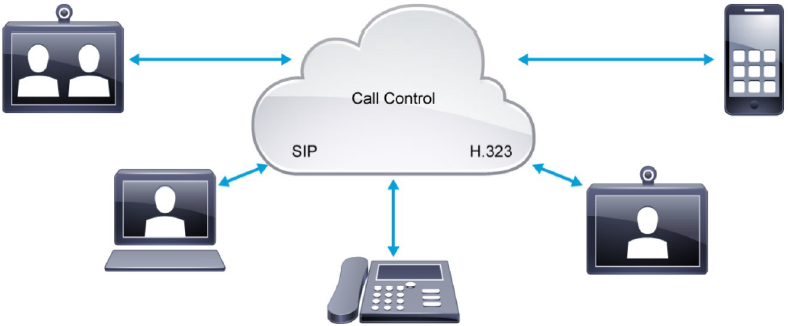
\includegraphics{img/fig_diagrama_simple_collab}
    \caption{Esquema simple de VoIP}
    \label{figura:fig_diagrama_simple_collab}
  \end{figure}
\end{itemize}

En la actualidad existen cientos de códecs, muchos de ellos propietarios. SIP usa Session Description Protocol (SDP), que define en la cabecera de los mensajes de una conversación SIP todos los códeds soportados, los cuales están identificados por una cadena de caracteres y pueden ser registrados por cualquier persona. Esto hace que SIP pueda funcionar con cualquier códec. 

H323 se caracteriza sin embargo por requerir que cada códec esté registrado y estandarizado de forma centralizada, hecho que repercute en pequeñas desarrolladoras y universidades pues muchos traen propiedad intelectual; no existen los códecs sub-28.8Kb/s gratis que puedan ser usados en un sistema H323. Por todo ello, y gracias a su facilidad de implementación y adaptabilidad a la naturaleza evolutiva de Internet, SIP está ganando gran populariad, siendo el protocolo de elección en las soluciones de Cisco y Microsoft, entre otros. Además su  ``interfaz'' amigable al lenguaje humano permite hacer \emph{debugging} con mayor facilidad y legibilidad. 
Ambos protocolos son muy usados no obstante.
\\

\begin{table} [h]
  \begin{center}
    \begin{tabular}{| c | c |}
    \hline
    \textbf{H323} & \textbf{SIP} \\ \hline
    Extenso, complejo y rígido & Modular, flexible y extensible\\\hline
    Buena interoperabilidad por su rigidez & Fácilmente adaptable a nuevas funcionalidades\\\hline
    Codificación en binario & Codificación en ASCII \\\hline
    Direcciones por \emph{host} o \#tlf & Direcciones por URLs \\ \hline
    Q.931 sobre TCP & SIP sobre TCP/UDP \\\hline
    \end{tabular}
    \label{tabla:SIPvsH323}
    \caption{Comparativa entre SIP y H323}
  \end{center}
\end{table}
\subsection{SIP}
\label{sec:sip}
Tomando como referencia protocolos con un gran recorrido y un buen historial de evolución como HTTP y SMTP, SIP ha basado la lógica de sus flujos de comunicación con una estructura de petición -$>$ respuesta. Este flujo de de comunicación Resquest/Response (Figura~\ref{figura:fig_phones}) utiliza los llamados \emph{métodos} SIP, compuestos por un grupo reducido de sencillas cabeceras con nombres muy intuitivos.

\begin{figure}[h]
  \centering
  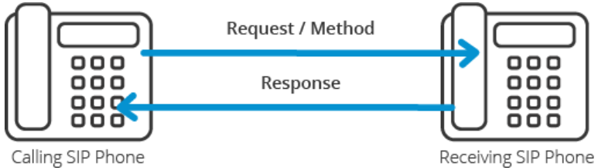
\includegraphics{img/fig_phones}
  \caption{Comunicación vía SIP entre dos terminales}
  \label{figura:fig_phones}
\end{figure}

De forma resumida, se puede decir que las más importantes son:
\begin{itemize}
  \item \textbf{INVITE}. Petición con la que un agente invita a otro a una sessión telefónica.
  \item \textbf{ACK}. Mensaje de respuesta de confirmación de recepción de la petición INVITE.
  \item \textbf{REGISTER}. Registra contra un servidor SIP la dirección listada en la cabecera ``To''.
  \item \textbf{BYE}. El cliente corta la conexión.\\
\end{itemize}

SIP generalmente trae consigo un protocolo de descripción de sesión, llamado SDP, cuyo propósito es transmitir información acerca de los streams de media para ayudar a los participantes a recolectar información sobre una llamada. Proporciona información acerca de la sesión, como el nombre y propósito de la sesón, información del medio, protocolos, formatos de códec, tiempo e información del transporte. Además, posee una estructura corta y visual con descripción textual, con entradas del tipo $<$type$>$ = $<$value$>$.

SDP permite a un participante consultar toda esta información antes de aceptar la invitación, de manera que puede decidir si unirse o no a la llamada, o determinar de qué manera y en qué momento unirse si decide hacerlo.

En la Figura~\ref{figura:fig_sip_flow} se puede ver un ejemplo de flujo SIP entre dos teléfonos IP. Entre ambos endpoints se encuentra un servidor SIP, que se encarga de registrar sus direcciones y reenviar las peticiones si tuviera también el papel de proxy. En este contexto, se pueden distinguir cuatros procesos:
\begin{enumerate}
  \item Proceso de registro de los agentes contra el servidor SIP para que otros agentes puedan localizarlos. Este proceso se realiza cuando los usuarios encienden su dispositivo, y así se quedan hasta que reciben o realizan una llamada.
  \item Proceso de invitación a sesión, el \emph{Tinder} de las comunicaciones VoIP. Agente1 manda la invitación al servidor SIP con la dirección de Agente2 en la cabecera ``To:''. El servidor SIP busca dicha dirección en su base de datos y una vez hay match, reenvía la petición a Agente2. Este elemento intermedio envía inmediatamente una respuesta 100 Trying a Agente1 para no comience retransmisiones de la petición INVITE. Si Agente2 acepta la llamada, comienza la transmisión de la petición 180 Ringing, a la que seguirá una respuesta 200 OK. Una vez Agente1 recibe el 200 OK, envía una petición ACK, dando luegar al siguiente proceso.
  \item Establecimiento de sesión. Comienza la transmisión punto a punto de paquetes vía RTP, ya sea para audio o vídeo. El servidor SIP no tiene cabida en este escenario, pues se ha creado una conversación privada entre los dos usuarios.
  \item Cuando un agente desea colgar, envía una petición BYE al servidor, el cual la retransmitirá a Agente2. A Agente2 no le quedará otra que aceptar la finalización de sesión y devolver una respuesta 200 OK, retransmitida a Agente1.
\end{enumerate}

\begin{figure}
  \centering
  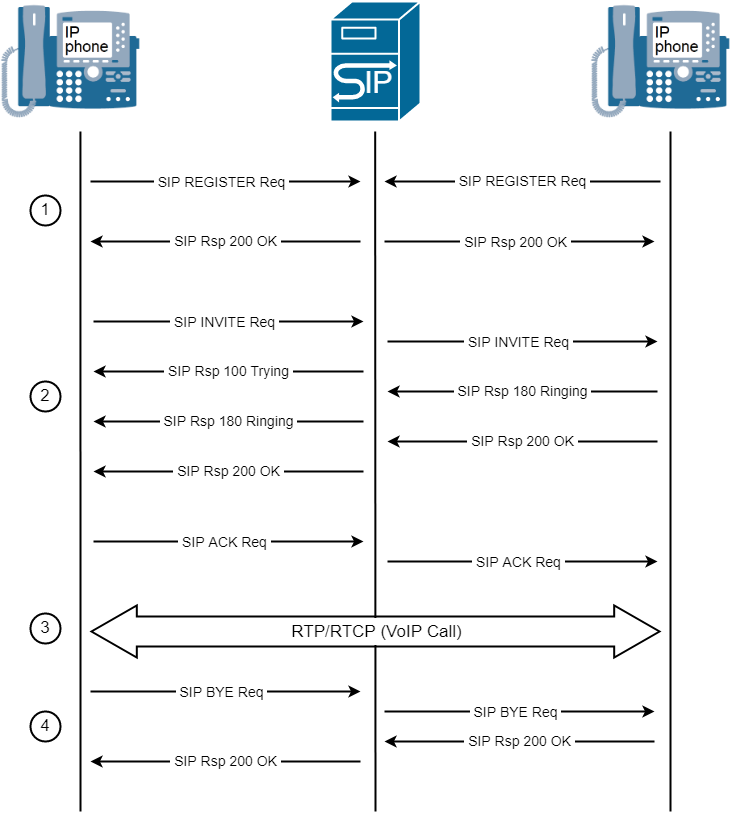
\includegraphics{img/fig_sip_flow}
  \caption{Flujo básico SIP}
  \label{figura:fig_sip_flow}
\end{figure}




\subsection{Tecnologías complementarias}
\label{sec:tecnologias-complementarias}
Junto a SIP, Cisco usa un protocolo propietario de control de terminal, nombrado Skinny Call Control Protocol (SCCP) comúnmente llamado Skinny, para la comunicación entre el Call Manager y clientes ligeros, tales como los teléfonos IP. Este protocolo fue desarrollado inicialemente por Selsius Corporation, empresa adquirida por Cisco en 1998. La labor de este protocolo ha quedado relegada a una cantidad pequeña de tareas, como la especificacion de recrusos de media o la comunicación opcional con equipos analógicos. \\Actualmente, todos los nuevos teléfonos IP funcionan con SIP.
\\

\begin{figure}[h]
  \centering
  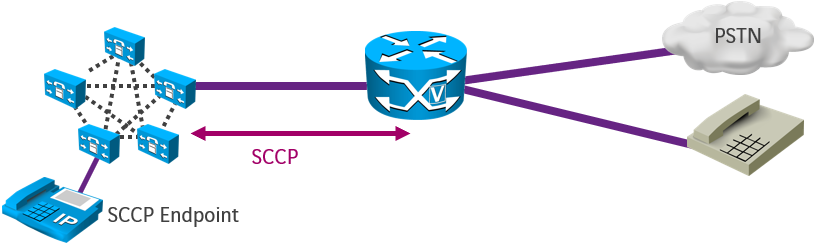
\includegraphics{img/fig_skinny}
  \caption{Flujo de comunicación por SCCP}
  \label{figura:fig_skinny}
\end{figure}


-------------------------------------------------------------

Puedes citar libros, como el de Bonabeau et al., sobre procesos estigmérgicos~\cite{Cisco:_video}.
Me encantan los procesos estigmérgicos.
Deberías leer más sobre ellos.
Pero quizás no ahora, que tenemos que terminar la memoria para sacarnos por fin el título.
Nota que el \~ \ añade un espacio en blanco, pero no deja que exista un salto de línea.
Imprescindible ponerlo para las citas.

Citar es importantísimo en textos científico-técnicos.
Porque no partimos de cero.
Es más, partir de cero es de tontos; lo suyo es aprovecharse de lo ya existente para construir encima y hacer cosas más sofisticadas.
¿Dónde puedo encontrar textos científicos que referenciar?
Un buen sitio es Google Scholar: {http://scholar.google.com}.
Por ejemplo, si buscas por ``stigmergy libre software'' para encontrar trabajo sobre software libre y el concepto de \emph{estigmergia} (¿te he comentado que me gusta el concepto de estigmergia ya?), encontrarás un artículo que escribí hace tiempo cuyo título es ``Self-organized development in libre software: a model based on the stigmergy concept''.
Si pulsas sobre las comillas dobles (entre la estrella y el ``citado por ...'', justo debajo del extracto del resumen del artículo, te saldrá una ventana emergente con cómo citar.
Abajo a la derecha, aparece un enlace BibTeX.
Púlsalo y encontrarás la referencia en formato BibTeX, tal que así:

{\footnotesize
\begin{verbatim}
@inproceedings{robles2005self,
  title={Self-organized development in libre software:
         a model based on the stigmergy concept},
  author={Robles, Gregorio and Merelo, Juan Juli\'an
          and Gonz\'alez-Barahona, Jes\'us M.},
  booktitle={ProSim'05},
  year={2005}
}
\end{verbatim}
}

Copia el texto en BibTeX y pégalo en el fichero \texttt{memoria.bib}, que es donde están las referencias bibliográficas.
Para incluir la referencia en el texto de la memoria, deberás citarlo, como hemos hecho antes con~\cite{bonabeau:_swarm}, lo que pasa es que en vez de el identificador de la cita anterior (bonabeau:\_swarm), tendrás que poner el nuevo (robles2005self).
Compila el fichero \texttt{memoria.tex} (\texttt{pdflatex memoria.tex}), añade la bibliografía (\texttt{bibtex memoria.aux}) y vuelve a compilar \texttt{memoria.tex} (\texttt{pdflatex memoria.tex})\ldots y \emph{voilà} ¡tenemos una nueva cita~%\cite{robles2005self}!

También existe la posibilidad de poner notas al pie de página, por ejemplo, una para indicarte que visite la página del GSyC\footnote{\url{http://gsyc.es}}.


-------------------------------------------------------------


%%%%%%%%%%%%%%%%%%%%%%%%%%%%%%%%%%%%%%%%%%%%%%%%%%%%%%%%%%%%%%%%%%%%%%%%%%%%%%%%
%%%%%%%%%%%%%%%%%%%%%%%%%%%%%%%%%%%%%%%%%%%%%%%%%%%%%%%%%%%%%%%%%%%%%%%%%%%%%%%%
% DISEÑO E IMPLEMENTACIÓN %
%%%%%%%%%%%%%%%%%%%%%%%%%%%%%%%%%%%%%%%%%%%%%%%%%%%%%%%%%%%%%%%%%%%%%%%%%%%%%%%%

\cleardoublepage
\chapter{Diseño e implementación}

De acuerdo a los contratos legales establecidos entre mi empresa (ejecutora del proyecto) y el cliente (receptora), no me está permitido hacer una reproducción de la solución con un detalle exacto, pero sí puedo definir de forma aproximada una arquitectura funcional similar, intentando reflejar todas mis tareas ejecutadas durante la instalación.

\section{Arquitectura general}
\label{sec:arquitectura}

En la figura ~\ref{figura:fig_arquitectura} se muestra un esquema simplificado de la solución, presentando 4 zonas delimitadas. 

Empezando desde arriba, la primera zona representa la red pública de telefonía (PSTN), desde la que una persona puede realizar una llamada desde su teléfono móvil o fijo al número de atención al cliente definido para la entrada al sistema. También tenemos una pequeña nube representando el \emph{Busines to Business}, que en este caso son empresas con su propia red de telefonía privada conectadas a la solución de este proyecto mediante un elemento intermedio de control de fronteras: el SBC.

En la segunda zona, sobrepasando el primer borde de control, podemos diferenciar dos capas imaginarias:
\begin{itemize}
  \item Capa de conectividad, donde están ubicados el Gateway de voz y el SBC, ambos elementos físicos. Sus funciones serán enrutar las llamadas hacia la PSTN (a través del Gateway) y enviar las llamadas a los clientes ubicados en las redes privadas de los clientes (a través del SBC).
  \item Capa de servicios, donde se encuentran los servidores físicos que almacenan las máquinas virtuales de estos elementos. Sus funciones serán aplicar, entre otras, toda la lógica de gestión de llamadas entrantes y salientes, la configuración necesaria de interconexionado entre máquinas o las grabaciones de usuarios. El elemento más importante aquí es el Call Manager, que interactúa directamente con el resto de elementos.
  \item En la tercera zona, delimitada por dos firewalls y llamada también Zona Desmilitarizada (DMZ), se encuentra un servidor proxy propietario de Cisco con funciones especiales, ya que es el elemento que hace posible el login a la plataforma desde ubicaciones externas a la red privada por parte de los agentes. Esta zona está especialmente diseñada para alojar proxys en su interior, pues tiene la característica de permitir tráfico hacia el exterior pero bloquearlo hacia la red interna. Podría decirse que es como el jardín de una casa, donde se pueden colocar ciertos objetos, pero los de mayor valor se guardan dentro.
  \item Por último, al otro lado del firewall externo, se encuentra la red de Internet. Los agentes se encuentran en esta zona y hacen login a la plataforma desde su domicilio o desde su oficina de trabajo.
\end{itemize}

\begin{figure}[h]
  \centering
  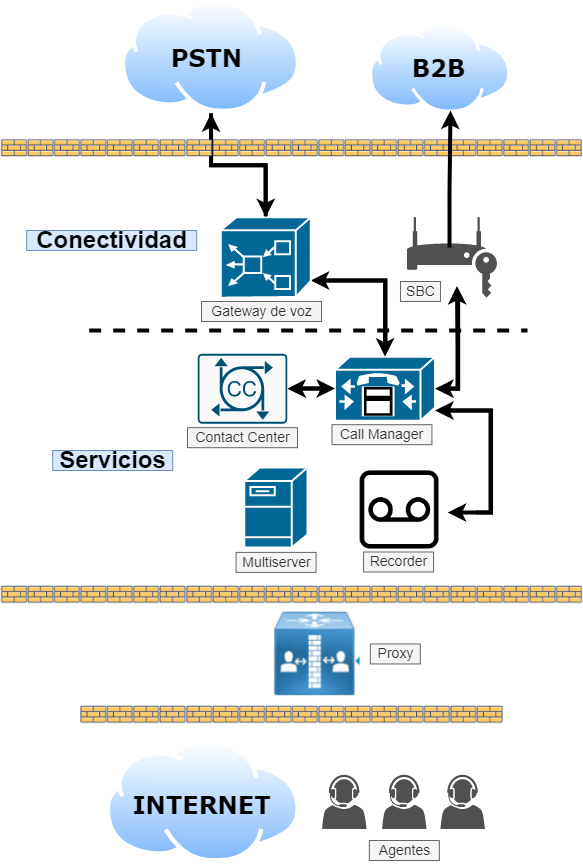
\includegraphics[scale=0.55]{img/fig_arquitectura}
  \caption{Diseño a alto nivel de la arquitectura montada}
  \label{figura:fig_arquitectura}
\end{figure}

\section{Alcance y casos de uso}
\label{sec:alcance}
Los elementos implicados en la solución son los siguientes:
\begin{itemize}
  \item \textbf{Call Manager}. Al ser una solucón redundada, necesitará tener un elemento \emph{master} y otro \emph{slave}.
  \item \textbf{Cisco Unified Presence}. Servidores de presencia, serán \emph{slaves} del Call Manager \emph{master}.
  \item \textbf{Jabber}. Cliente Cisco para llamadas, videoconferencias, mensajería y compartición de escritorio.
  \item \textbf{Contact Center}. Servidor UCCX que aloja el aplicativo Finesse. Consta de varios nodos al estar geográficamente redundado.
  \item \textbf{Proxy}. Gateway para enrutamiento de llamadas desde internet al Call Manager. Se usa también para habilitar la funcionalidad MRA (Mobile and Remote Access).
\end{itemize}

\section{Configuración de los componentes}
\label{sec:config}

\subsection{Virtualización}
\label{sec:vmware}
Los servidores físicos se configuraron inicialmente con los ajustes de red básicos, que son la IP, la máscara de subred y el gateway. Sobre esta capa de configuracion, está instalado el aplicativo de virtualización llamado VMWare. 

VMWare es una solución basada en el acceso a un escritorio remoto que permite a los usuarios ejecutar máquinas virtuales. Se trata de un sistema que permite operar con software, emulando a un sistema físico (un computador, un hardware, etc.). Esta plataforma permite dividir un único servidor físico en múltiples máquinas virtuales.

Se utilizan funciones especiales en CPU x86 de 64 bits modernas para crear máquinas virtuales seguras y completamente aisladas que encapsulan un sistema operativo y sus aplicaciones. La capa de virtualización de VMware asigna los recursos de hardware físicos a los recursos virtuales de la máquina virtual, por lo que cada máquina virtual cuenta con una CPU, una memoria, unos discos y unos dispositivos de E/S propios, y equivale en su totalidad a una máquina x86 convencional. VMware Workstation, que es el hipervisor de escritorio, se ha instalado en el sistema operativo host. Con ello se consigue una amplia compatibilidad de hardware al heredar del host la conciliación con los dispositivos.

En la Figura ~\ref{figura:fig_vmware} se presenta el aspecto de la interfaz del aplicativo con varias de las máquinas virtuales instaladas y parte de la información sensible ocultada.

\begin{figure}[h]
  \centering
  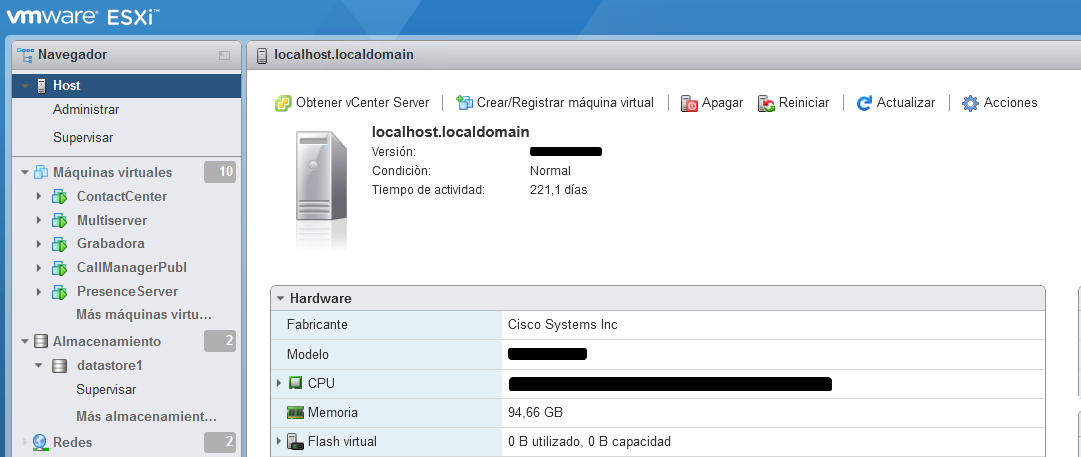
\includegraphics[scale=0.8]{img/fig_vmware}
  \caption{Interfaz web de VMWare}
  \label{figura:fig_vmware}
\end{figure}

\subsection{Call Manager}
\label{sec:call_manager}



%%%%%%%%%%%%%%%%%%%%%%%%%%%%%%%%%%%%%%%%%%%%%%%%%%%%%%%%%%%%%%%%%%%%%%%%%%%%%%%%
%%%%%%%%%%%%%%%%%%%%%%%%%%%%%%%%%%%%%%%%%%%%%%%%%%%%%%%%%%%%%%%%%%%%%%%%%%%%%%%%
% EXPERIMENTOS Y VALIDACIÓN %
%%%%%%%%%%%%%%%%%%%%%%%%%%%%%%%%%%%%%%%%%%%%%%%%%%%%%%%%%%%%%%%%%%%%%%%%%%%%%%%%

\cleardoublepage
\chapter{Experimentos y validación}

Este capítulo se introdujo como requisito en 2019.
Describe los experimentos y casos de test que tuviste que implementar para validar tus resultados.
Incluye también los resultados de validación que permiten afirmar que tus resultados son correctos.


%%%%%%%%%%%%%%%%%%%%%%%%%%%%%%%%%%%%%%%%%%%%%%%%%%%%%%%%%%%%%%%%%%%%%%%%%%%%%%%%
%%%%%%%%%%%%%%%%%%%%%%%%%%%%%%%%%%%%%%%%%%%%%%%%%%%%%%%%%%%%%%%%%%%%%%%%%%%%%%%%
% RESULTADOS %
%%%%%%%%%%%%%%%%%%%%%%%%%%%%%%%%%%%%%%%%%%%%%%%%%%%%%%%%%%%%%%%%%%%%%%%%%%%%%%%%

\cleardoublepage
\chapter{Resultados}

En este capítulo se incluyen los resultados de tu trabajo fin de grado.

Si es una herramienta de análisis lo que has realizado, aquí puedes poner ejemplos de haberla utilizado para que se vea su utilidad.


%%%%%%%%%%%%%%%%%%%%%%%%%%%%%%%%%%%%%%%%%%%%%%%%%%%%%%%%%%%%%%%%%%%%%%%%%%%%%%%%
%%%%%%%%%%%%%%%%%%%%%%%%%%%%%%%%%%%%%%%%%%%%%%%%%%%%%%%%%%%%%%%%%%%%%%%%%%%%%%%%
% CONCLUSIONES %
%%%%%%%%%%%%%%%%%%%%%%%%%%%%%%%%%%%%%%%%%%%%%%%%%%%%%%%%%%%%%%%%%%%%%%%%%%%%%%%%

\cleardoublepage
\chapter{Conclusiones}
\label{chap:conclusiones}


\section{Consecución de objetivos}
\label{sec:consecucion-objetivos}

Esta sección es la sección espejo de las dos primeras del capítulo de objetivos, donde se planteaba el objetivo general y se elaboraban los específicos.

Es aquí donde hay que debatir qué se ha conseguido y qué no.
Cuando algo no se ha conseguido, se ha de justificar, en términos de qué problemas se han encontrado y qué medidas se han tomado para mitigar esos problemas.

Y si has llegado hasta aquí, siempre es bueno pasarle el corrector ortográfico, que las erratas quedan fatal en la memoria final.
Para eso, en Linux tenemos aspell, que se ejecuta de la siguiente manera desde la línea de \emph{shell}:

\begin{verbatim}
  aspell --lang=es_ES -c memoria.tex
\end{verbatim}

\section{Aplicación de lo aprendido}
\label{sec:aplicacion}

Aquí viene lo que has aprendido durante el Grado/Máster y que has aplicado en el TFG/TFM. Una buena idea es poner las asignaturas más relacionadas y comentar en un párrafo los conocimientos y habilidades puestos en práctica.

\begin{enumerate}
  \item a
  \item b
\end{enumerate}


\section{Lecciones aprendidas}
\label{sec:lecciones_aprendidas}

Aquí viene lo que has aprendido en el Trabajo Fin de Grado/Máster.

\begin{enumerate}
  \item Aquí viene uno.
  \item Aquí viene otro.
\end{enumerate}


\section{Trabajos futuros}
\label{sec:trabajos_futuros}

Ningún proyecto ni software se termina, así que aquí vienen ideas y funcionalidades que estaría bien tener implementadas en el futuro.

Es un apartado que sirve para dar ideas de cara a futuros TFGs/TFMs.


%%%%%%%%%%%%%%%%%%%%%%%%%%%%%%%%%%%%%%%%%%%%%%%%%%%%%%%%%%%%%%%%%%%%%%%%%%%%%%%%
%%%%%%%%%%%%%%%%%%%%%%%%%%%%%%%%%%%%%%%%%%%%%%%%%%%%%%%%%%%%%%%%%%%%%%%%%%%%%%%%
% APÉNDICE(S) %
%%%%%%%%%%%%%%%%%%%%%%%%%%%%%%%%%%%%%%%%%%%%%%%%%%%%%%%%%%%%%%%%%%%%%%%%%%%%%%%%

\cleardoublepage
\appendix
\chapter{Manual de usuario}
\label{app:manual}

Esto es un apéndice.
Si has creado una aplicación, siempre viene bien tener un manual de usuario.
Pues ponlo aquí.

%%%%%%%%%%%%%%%%%%%%%%%%%%%%%%%%%%%%%%%%%%%%%%%%%%%%%%%%%%%%%%%%%%%%%%%%%%%%%%%%
%%%%%%%%%%%%%%%%%%%%%%%%%%%%%%%%%%%%%%%%%%%%%%%%%%%%%%%%%%%%%%%%%%%%%%%%%%%%%%%%
% BIBLIOGRAFIA %
%%%%%%%%%%%%%%%%%%%%%%%%%%%%%%%%%%%%%%%%%%%%%%%%%%%%%%%%%%%%%%%%%%%%%%%%%%%%%%%%

\cleardoublepage

% Las siguientes dos instrucciones es todo lo que necesitas
% para incluir las citas en la memoria
\bibliographystyle{abbrv}
\bibliography{memoria}  % memoria.bib es el nombre del fichero que contiene
% las referencias bibliográficas. Abre ese fichero y mira el formato que tiene,
% que se conoce como BibTeX. Hay muchos sitios que exportan referencias en
% formato BibTeX. Prueba a buscar en http://scholar.google.com por referencias
% y verás que lo puedes hacer de manera sencilla.
% Más información:
% http://texblog.org/2014/04/22/using-google-scholar-to-download-bibtex-citations/

\end{document}
